\documentclass{article}

\usepackage[utf8]{inputenc}
\usepackage[english]{babel}
\usepackage[shortlabels]{enumitem}
\usepackage{amsthm, amssymb, mathtools, amsmath, bbm, mathrsfs,stmaryrd}
\usepackage[margin=3cm]{geometry}
\usepackage[parfill]{parskip}
\usepackage[hidelinks]{hyperref}
\usepackage{ebproof}
\usepackage{cleveref}

\usepackage{caption}
\usepackage{subcaption}
\usepackage{tikz}

\newcommand{\sequent}[2]{#1\Rightarrow#2}
\newcommand{\set}[1]{\left\{#1\right\}}
\newcommand{\setwith}[2]{\set{#1:#2}}

\theoremstyle{definition}
\newtheorem{question}{Exercise}
\newtheorem*{lemma}{Lemma}

\newenvironment{solution}{\begin{proof}[Solution]\renewcommand{\qedsymbol}{}}{\end{proof}}

\title{Homework Proof Theory}
\author{Jonas van der Schaaf}
\date{\today}

\begin{document}
\maketitle

\begin{question}
    Is the following an intuitionistic tautology:
    \[
        ((\neg\neg p\to p)\to (p\vee \neg p))\to (\neg p\vee\neg\neg p)?
    \]

    \begin{solution}
        No it is not a tautology. Consider the model \(\mathbb{M}\)
        \begin{figure}[ht]
            \centering
            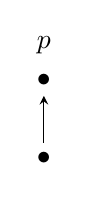
\begin{tikzpicture}
                \node (y) [label=\(p\)] {\(\bullet\)};
                \node (x) [below of = y] {\(\bullet\)};

                \draw [-stealth] (x) -- (y);
            \end{tikzpicture}
        \end{figure}
        Call the bottom node \(x\) and the top \(y\). Then clearly
        \(\mathbb{M},x\nvDash\neg p\) and \(\mathbb{M},x\nvDash\neg\neg p\),
        therefore \(\mathbb{M},x\nvDash\neg p\vee\neg\neg p\).

        If we show \(\mathbb{M},x\vDash((\neg\neg p\to p)\to (p\vee \neg p))\)
        this will show the formula is not a tautology.

        All classical tautologies hold on \(y\) because it sees no other point.
        Therefore \(\mathbb{M},y\vDash\neg\neg p\to p\) and \(\mathbb{M},y\vDash
        p\vee\neg p\), proving the implication in this point.

        At \(x\) the implication \((\neg\neg p\to p)\to (p\vee \neg p)\) is
        true. This is because both the antecedent and consequent of the
        implication are false at \(x\). This is easy to see because it is the
        classical counterexample to \(p\vee\neg p\) and similarly at \(x\) we
        know that \(\mathbb{M},x\nvDash p\) so it cannot satisfy \(\neg\neg p\)
        so the implication \(\neg\neg p\to p\) is true at \(x\) as well.

        This demonstrates the formula is not a tautology.
    \end{solution}
\end{question}
\end{document}